\section{Diagrama de Objetivos y Requerimientos}
\subsection{Diagrama general}
En este diagrama se muestra cuáles son los objetivos más grandes del proyecto, que se desarrollan en el resto de los diagramas.
\begin{figure}[H]
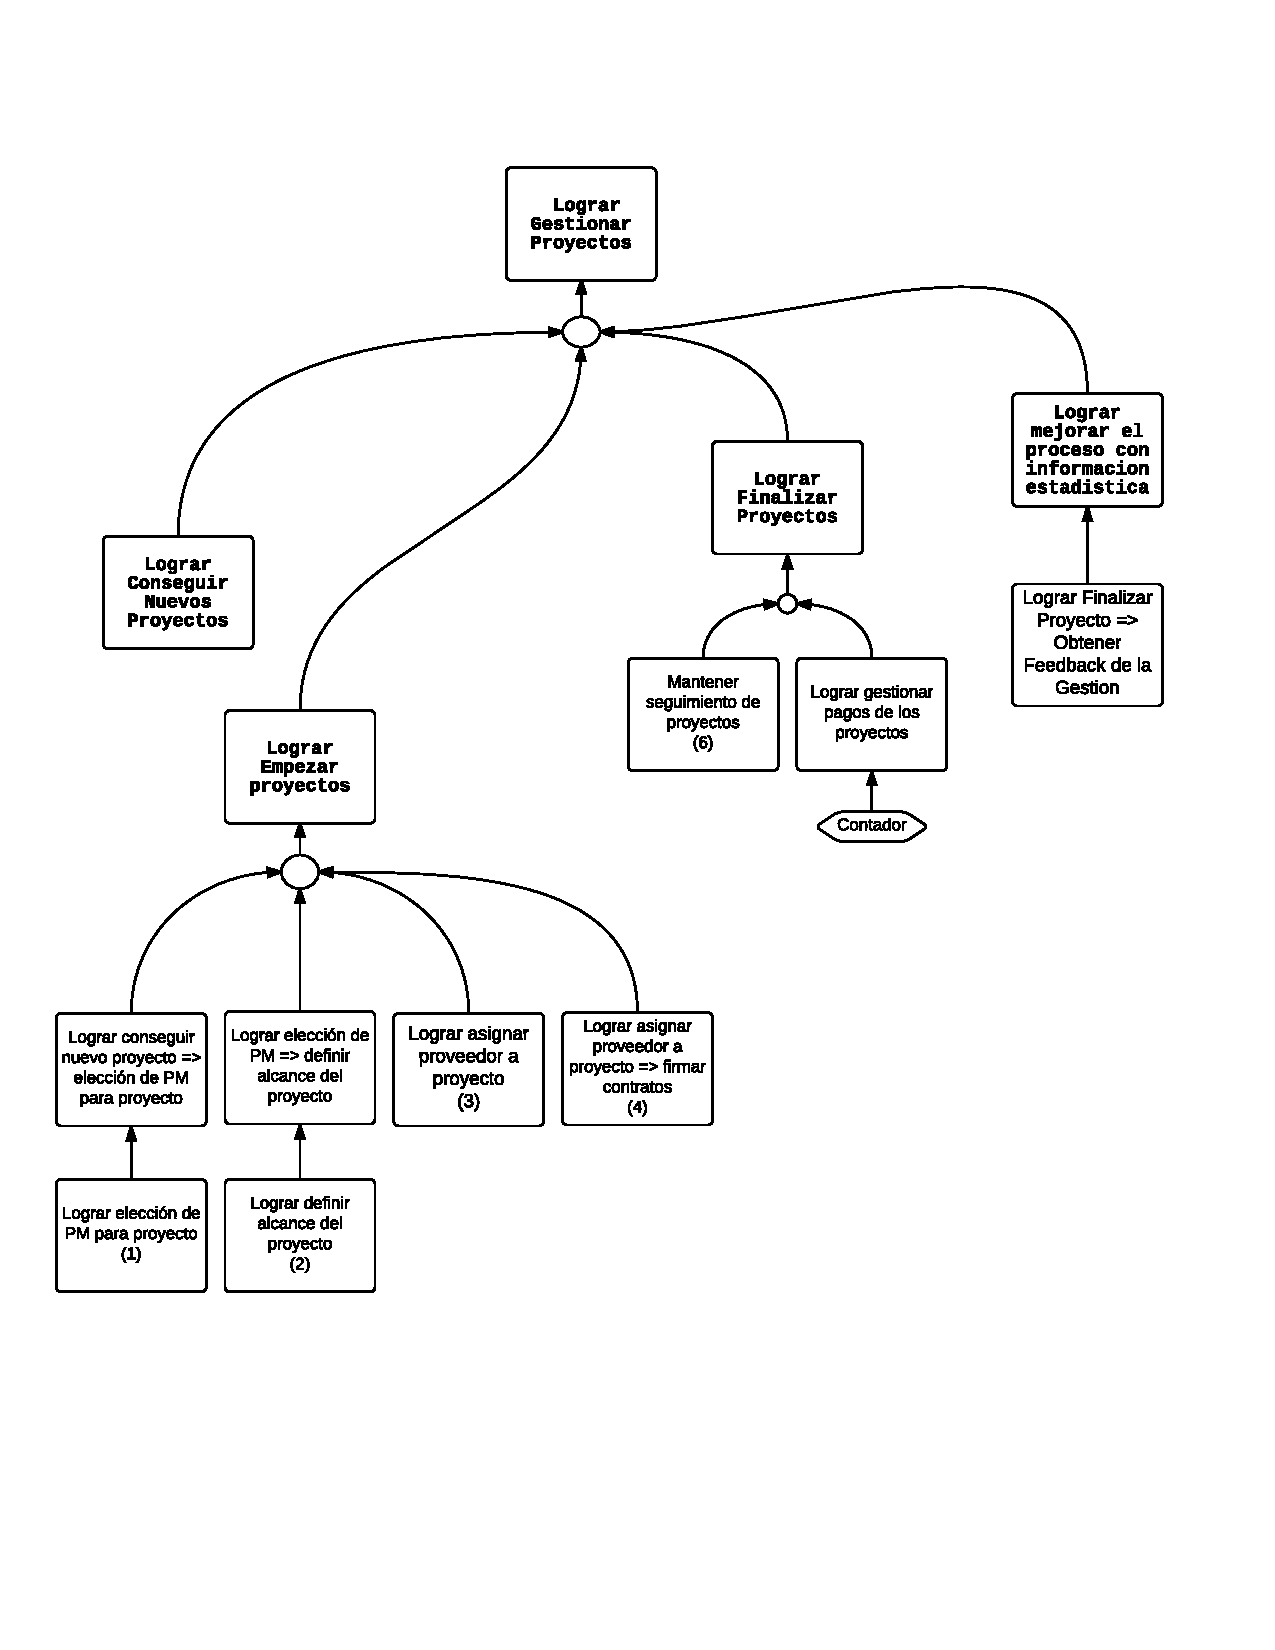
\includegraphics[width=\textwidth, clip=true, trim=15pt 170pt 15pt 80pt]{imagenes/objetivos/objetivos10.pdf}
\end{figure}
Podemos ver que los objetivos se dividen en los que permiten comenzar proyectos a partir de pre-proyectos, seguir proyectos en curso, conseguir nuevos proyectos (proveer herramientas para cargar preproyectos) y el circuito de feedback.

En particular el sistema de pagos no tiene que ver con el sistema, por lo tanto, no hay requerimientos de sistema que se vean en esta parte.

\subsection{Lograr Comenzar Nuevos Proyectos}
\begin{figure}[H]
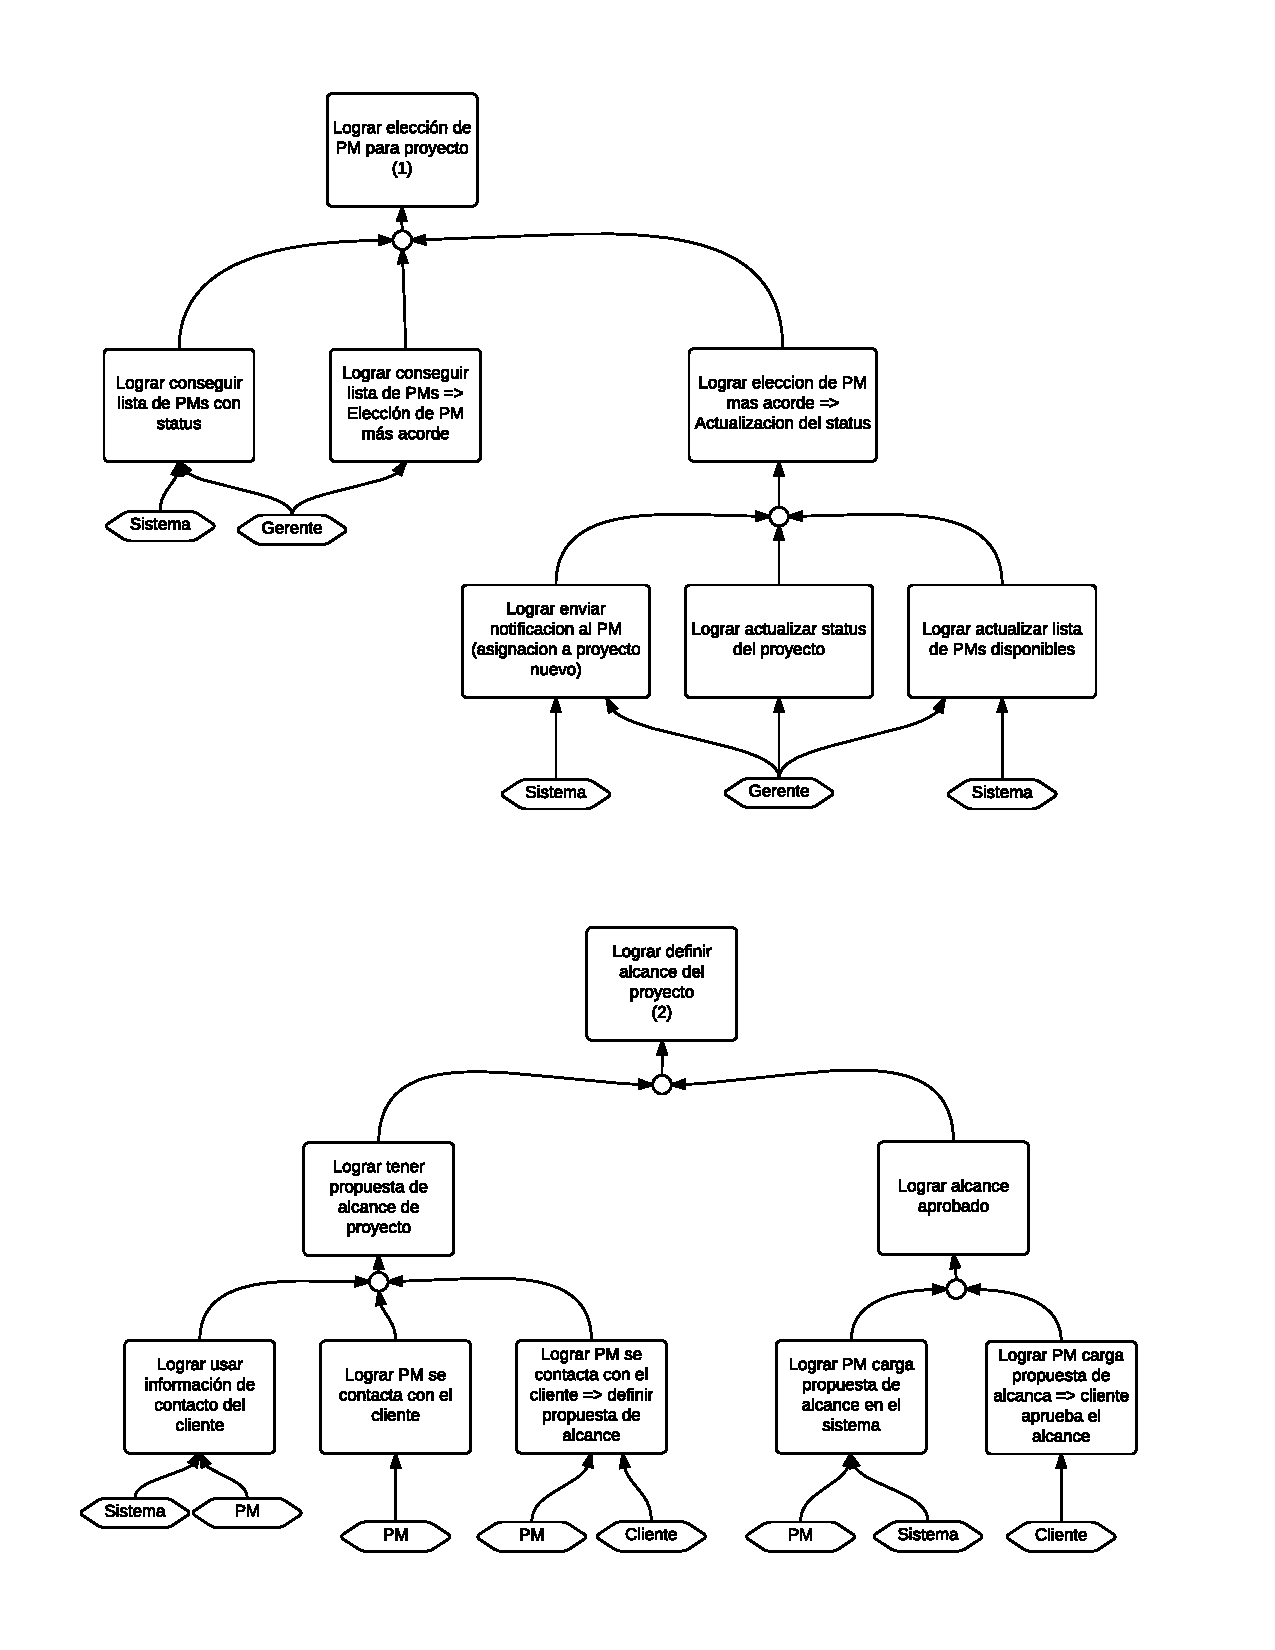
\includegraphics[width=\textwidth, clip=true, trim=15pt 0pt 15pt 0pt]{imagenes/objetivos/objetivos11.pdf}
\end{figure}
\begin{figure}[H]
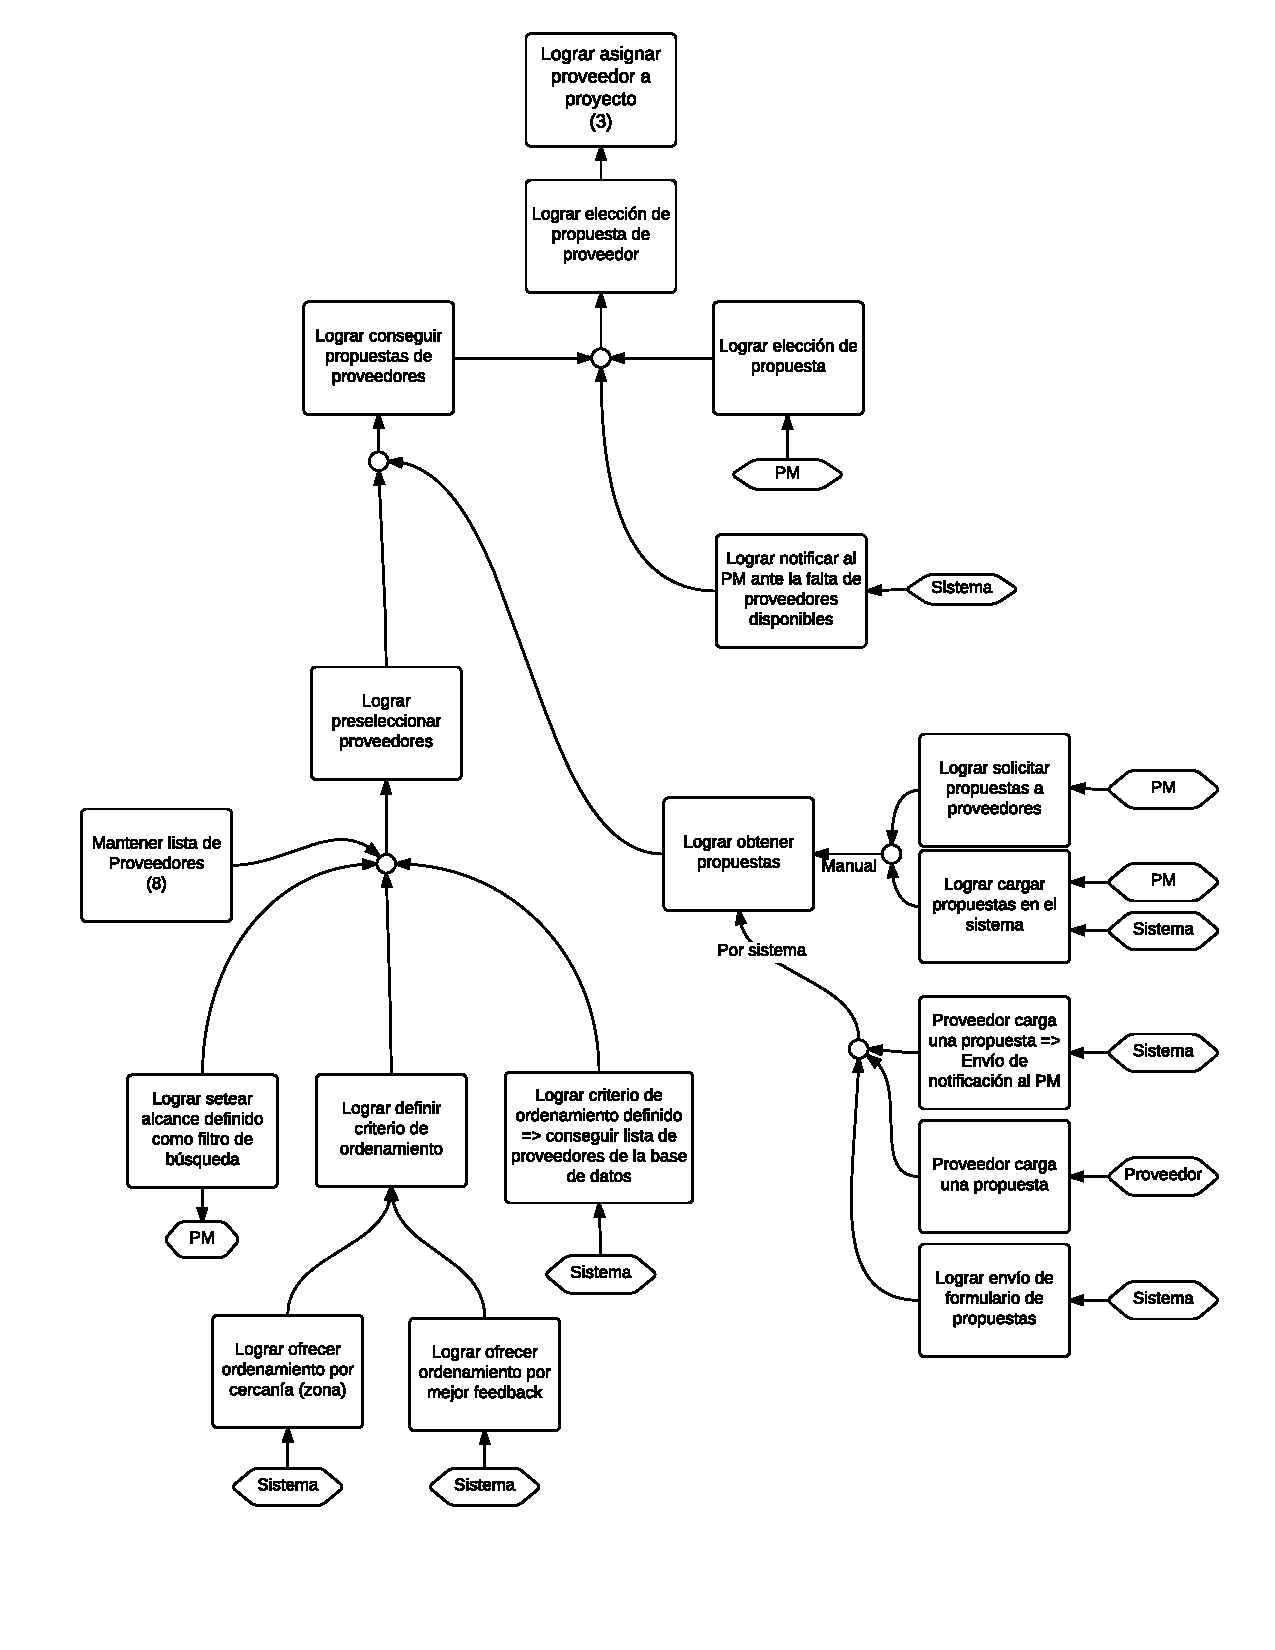
\includegraphics[width=\textwidth, clip=true, trim=15pt 0pt 15pt 0pt]{imagenes/objetivos/objetivos12.pdf}
\end{figure}
\begin{figure}[H]
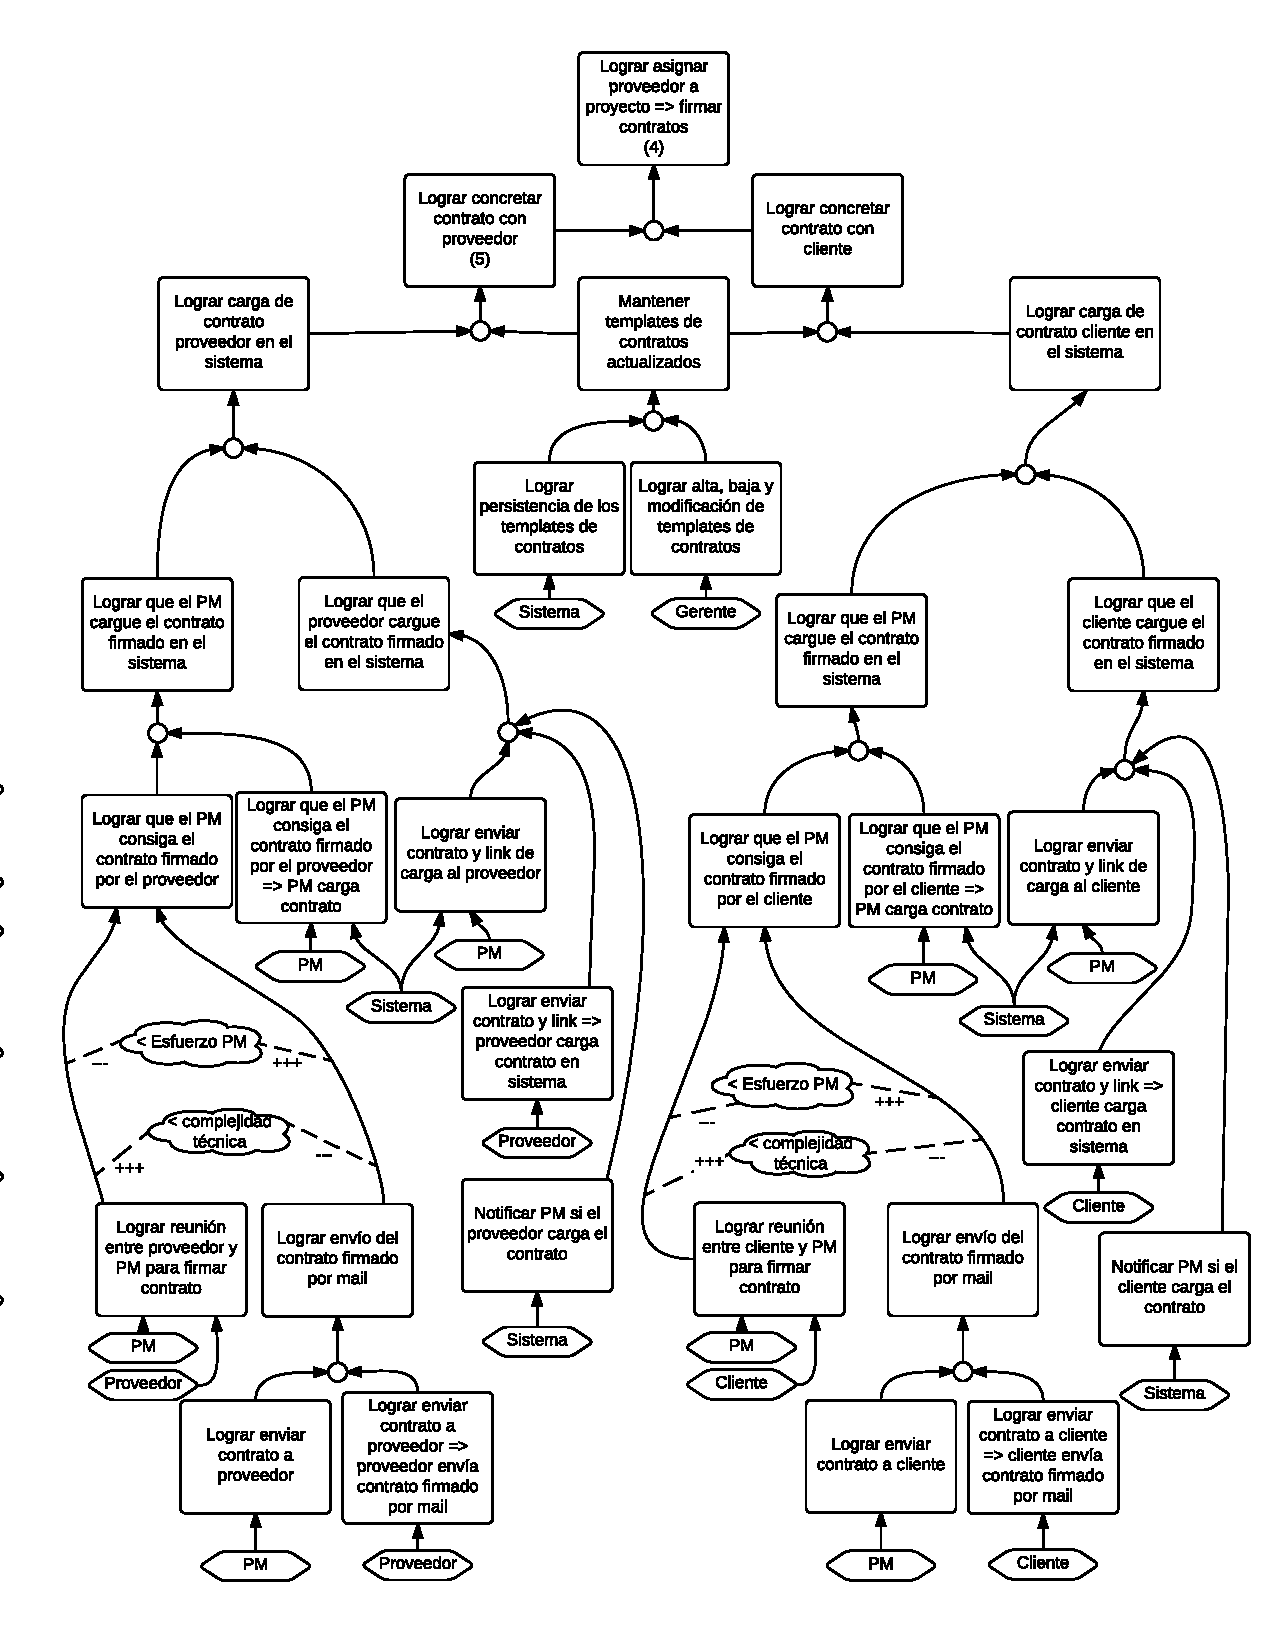
\includegraphics[width=\textwidth, clip=true, trim=15pt 0pt 15pt 0pt]{imagenes/objetivos/objetivos13.pdf}
\end{figure}

\subsubsection{Requerimientos de Sistema}
Los requerimientos para esta parte son:
\begin{itemize}
	\item En la asignación de PM:
	\begin{itemize}
		\item Ofrecer una lista de PMs con sus status
		\item Permitir al gerente asignar un PM a un proyecto %FALTA EN DIAGRAMA
		\item Enviar notificaciones al PM al ser asignado a proyecto nuevo
		\item Actualizar lista de PMs disponibles
	\end{itemize}
	\item En la definición del alcance:
	\begin{itemize}
		\item Ofrecer información de contacto del cliente
		\item Ofrecer al PM cargar propuestas de alcance
	\end{itemize}
	\item En la asignación de proveedor:
	\begin{itemize}
		\item Dado un criterio de ordenamiento, ofrecer lista de proveedores más relevantes
		\item Implementar filtros por zona y por puntaje
		\item Notificar si no hay un proveedor disponible
		\item Notificar obtención de proveedor %SACAR?
		\item Ofrecer al PM cargar propuestas en sistema
		\item Ofrecer al proveedor cargar propuestas en sistema mediante link de carga
		\item Notificar al PM ante una carga de propuesta de un proveedor
	\end{itemize}
	\item En la firma de contratos: % COMPLETAR
\end{itemize}

\subsection{Seguimiento de Proyectos}
\begin{figure}[H]
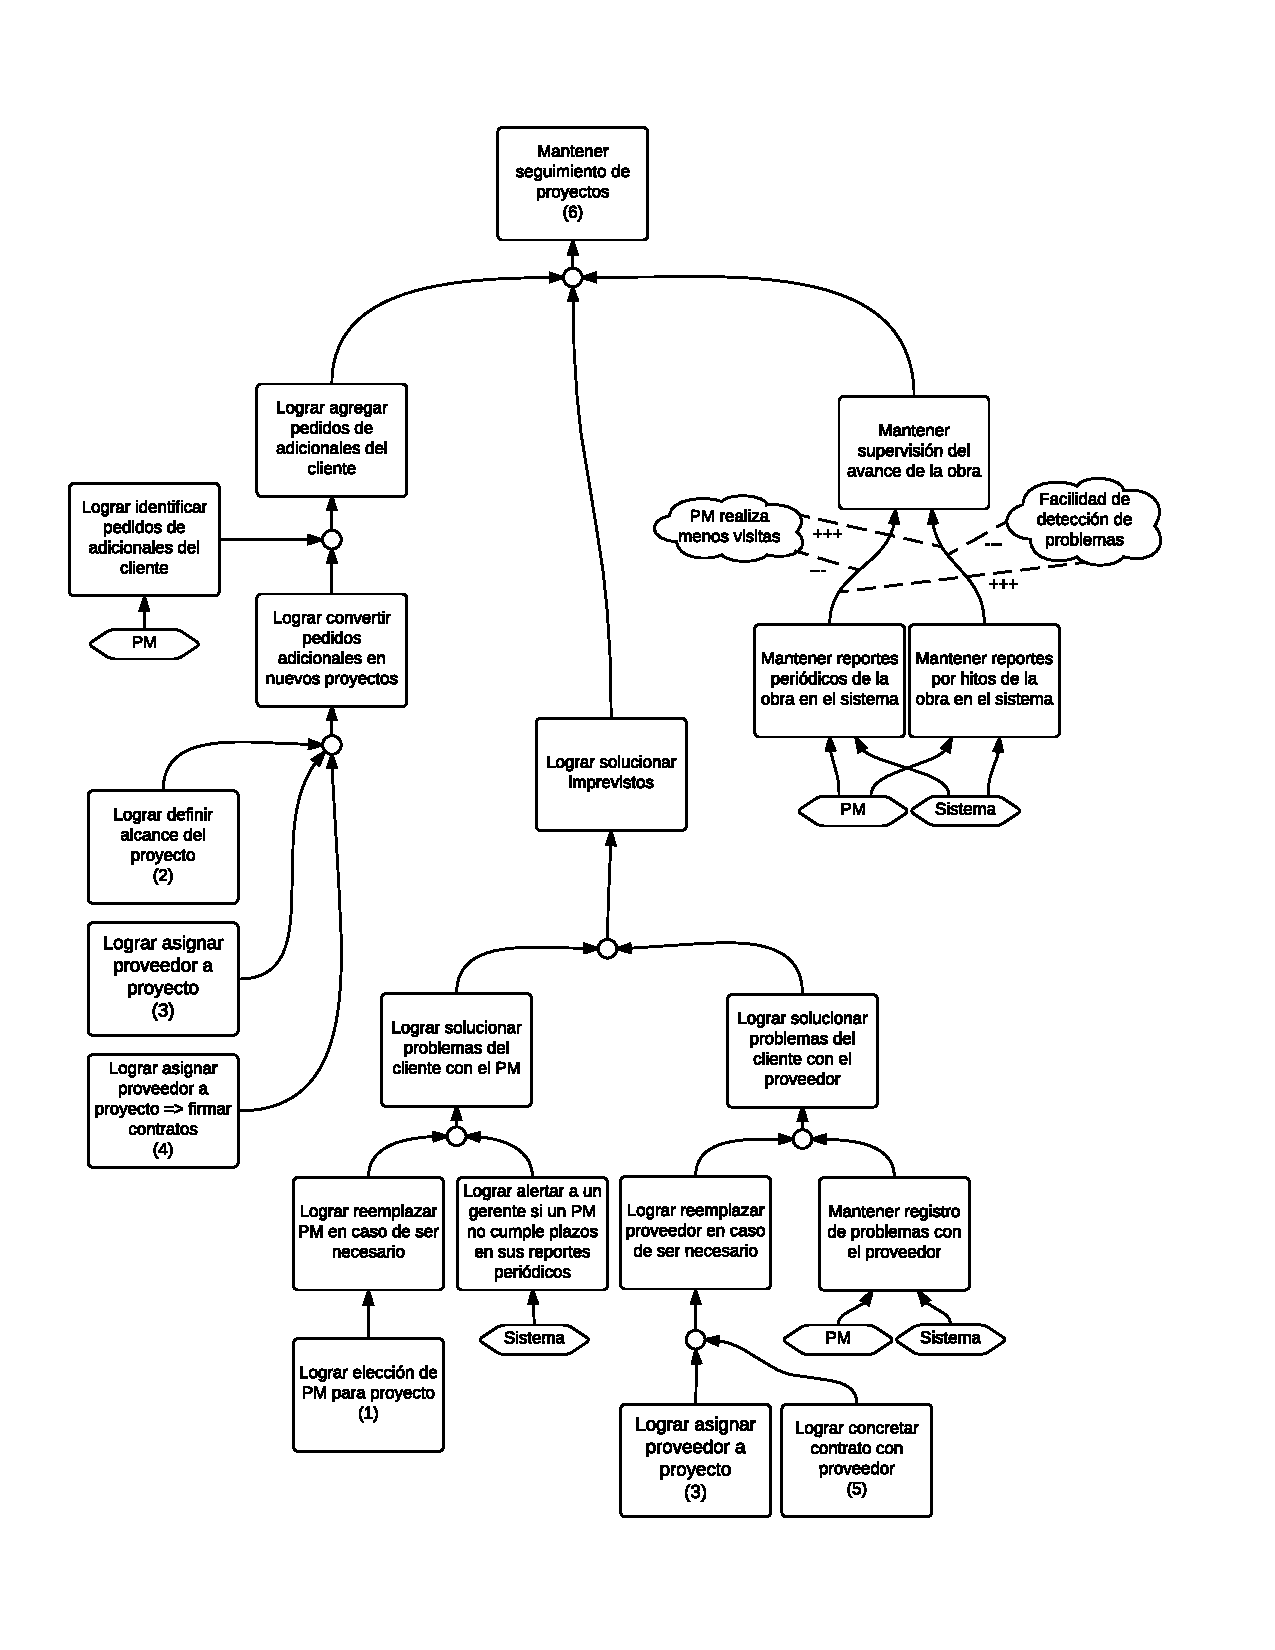
\includegraphics[width=\textwidth, clip=true, trim=15pt 0pt 15pt 0pt]{imagenes/objetivos/objetivos14.pdf}
\end{figure}

\subsection{Conseguir Nuevos Proyectos}
\begin{figure}[H]
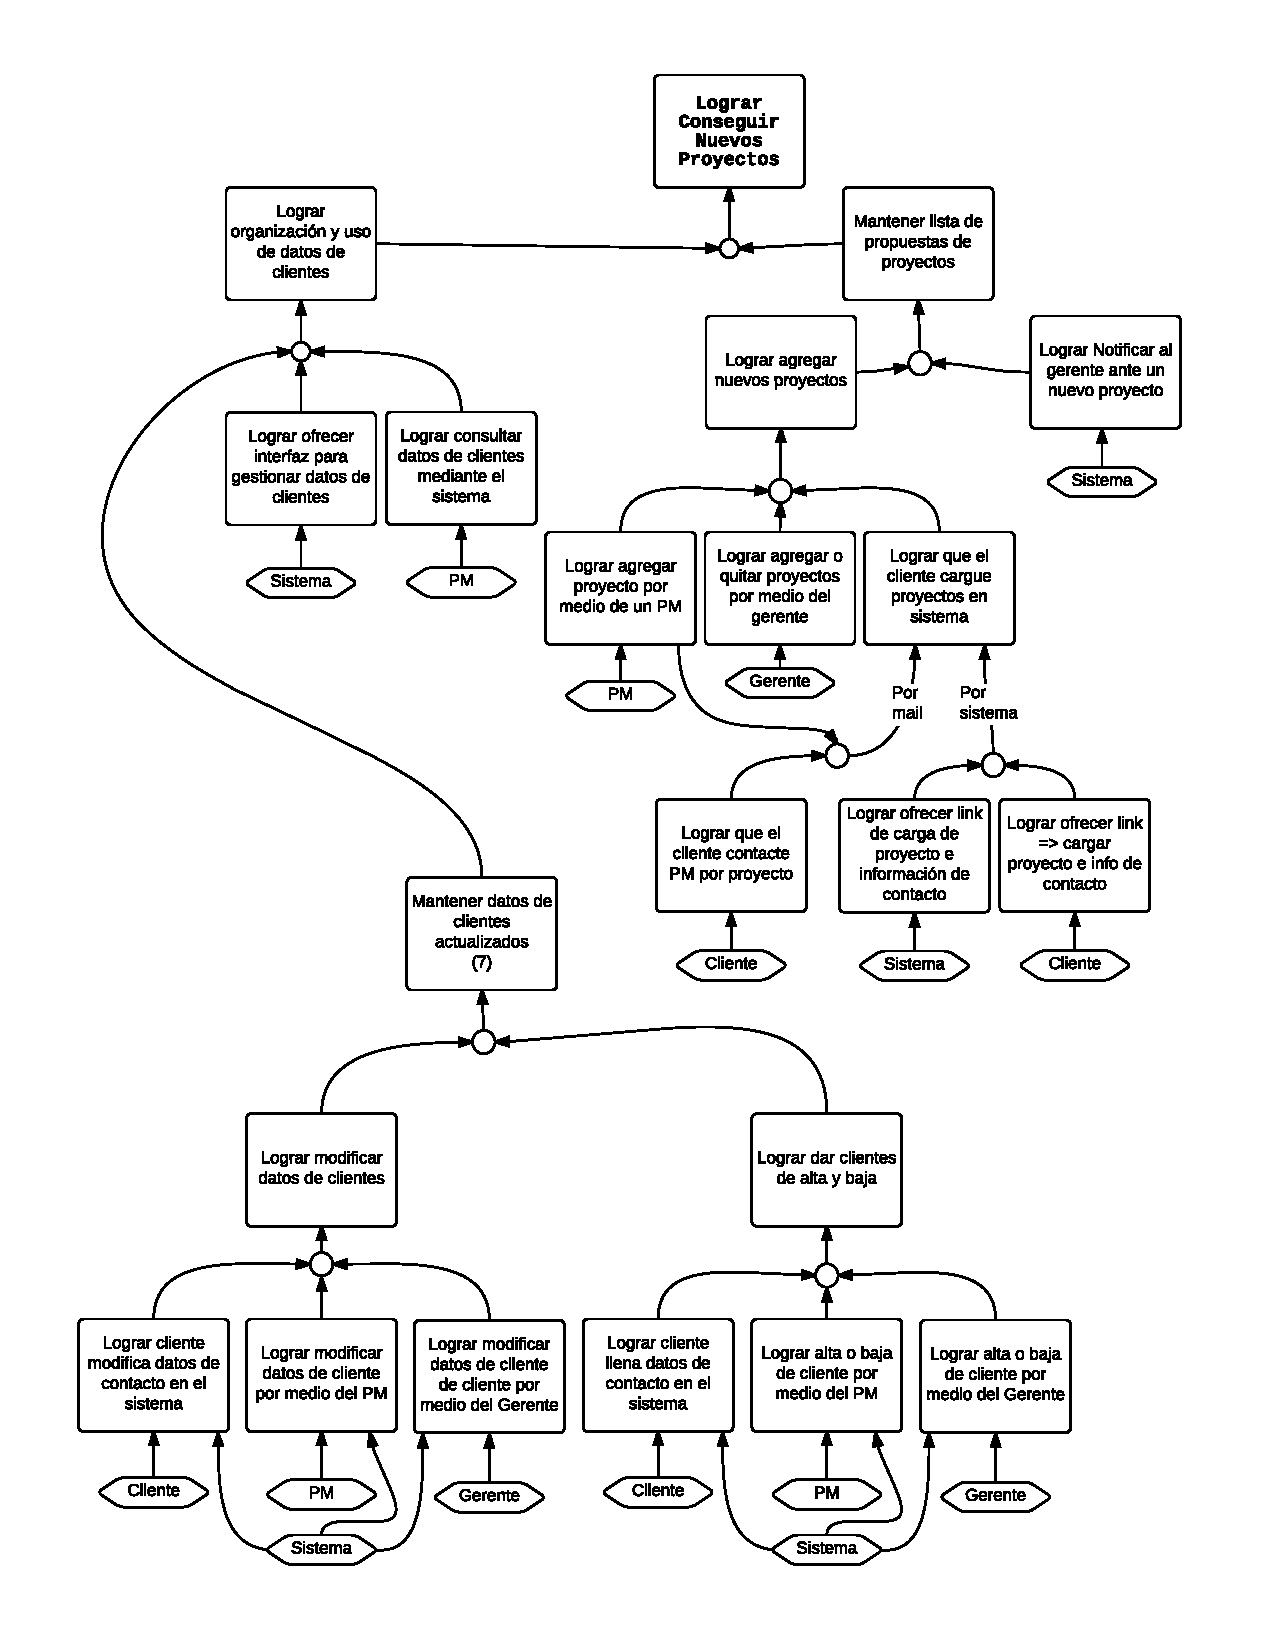
\includegraphics[width=\textwidth, clip=true, trim=15pt 0pt 15pt 0pt]{imagenes/objetivos/objetivos15.pdf}
\end{figure}
\begin{figure}[H]
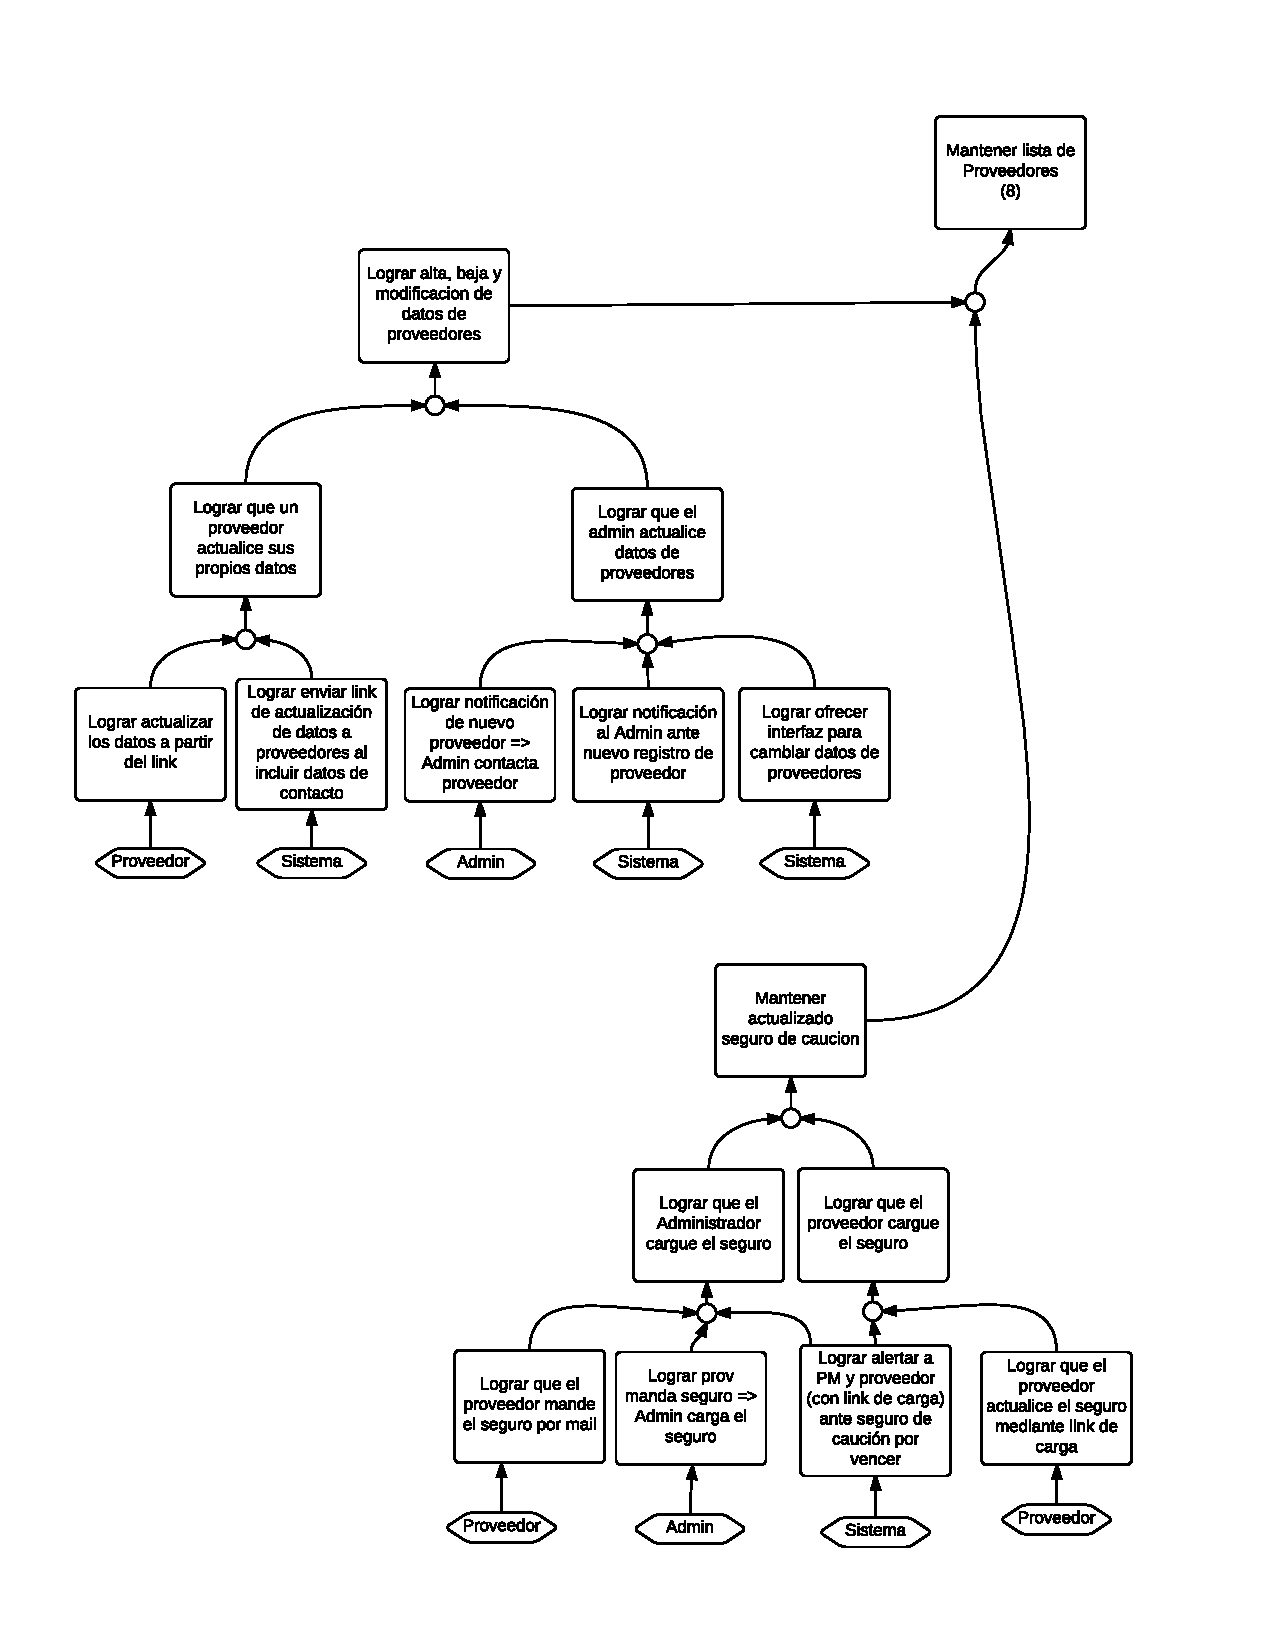
\includegraphics[width=\textwidth, clip=true, trim=15pt 0pt 15pt 0pt]{imagenes/objetivos/objetivos16.pdf}
\end{figure}

\subsection{Feedback}
\begin{figure}[H]
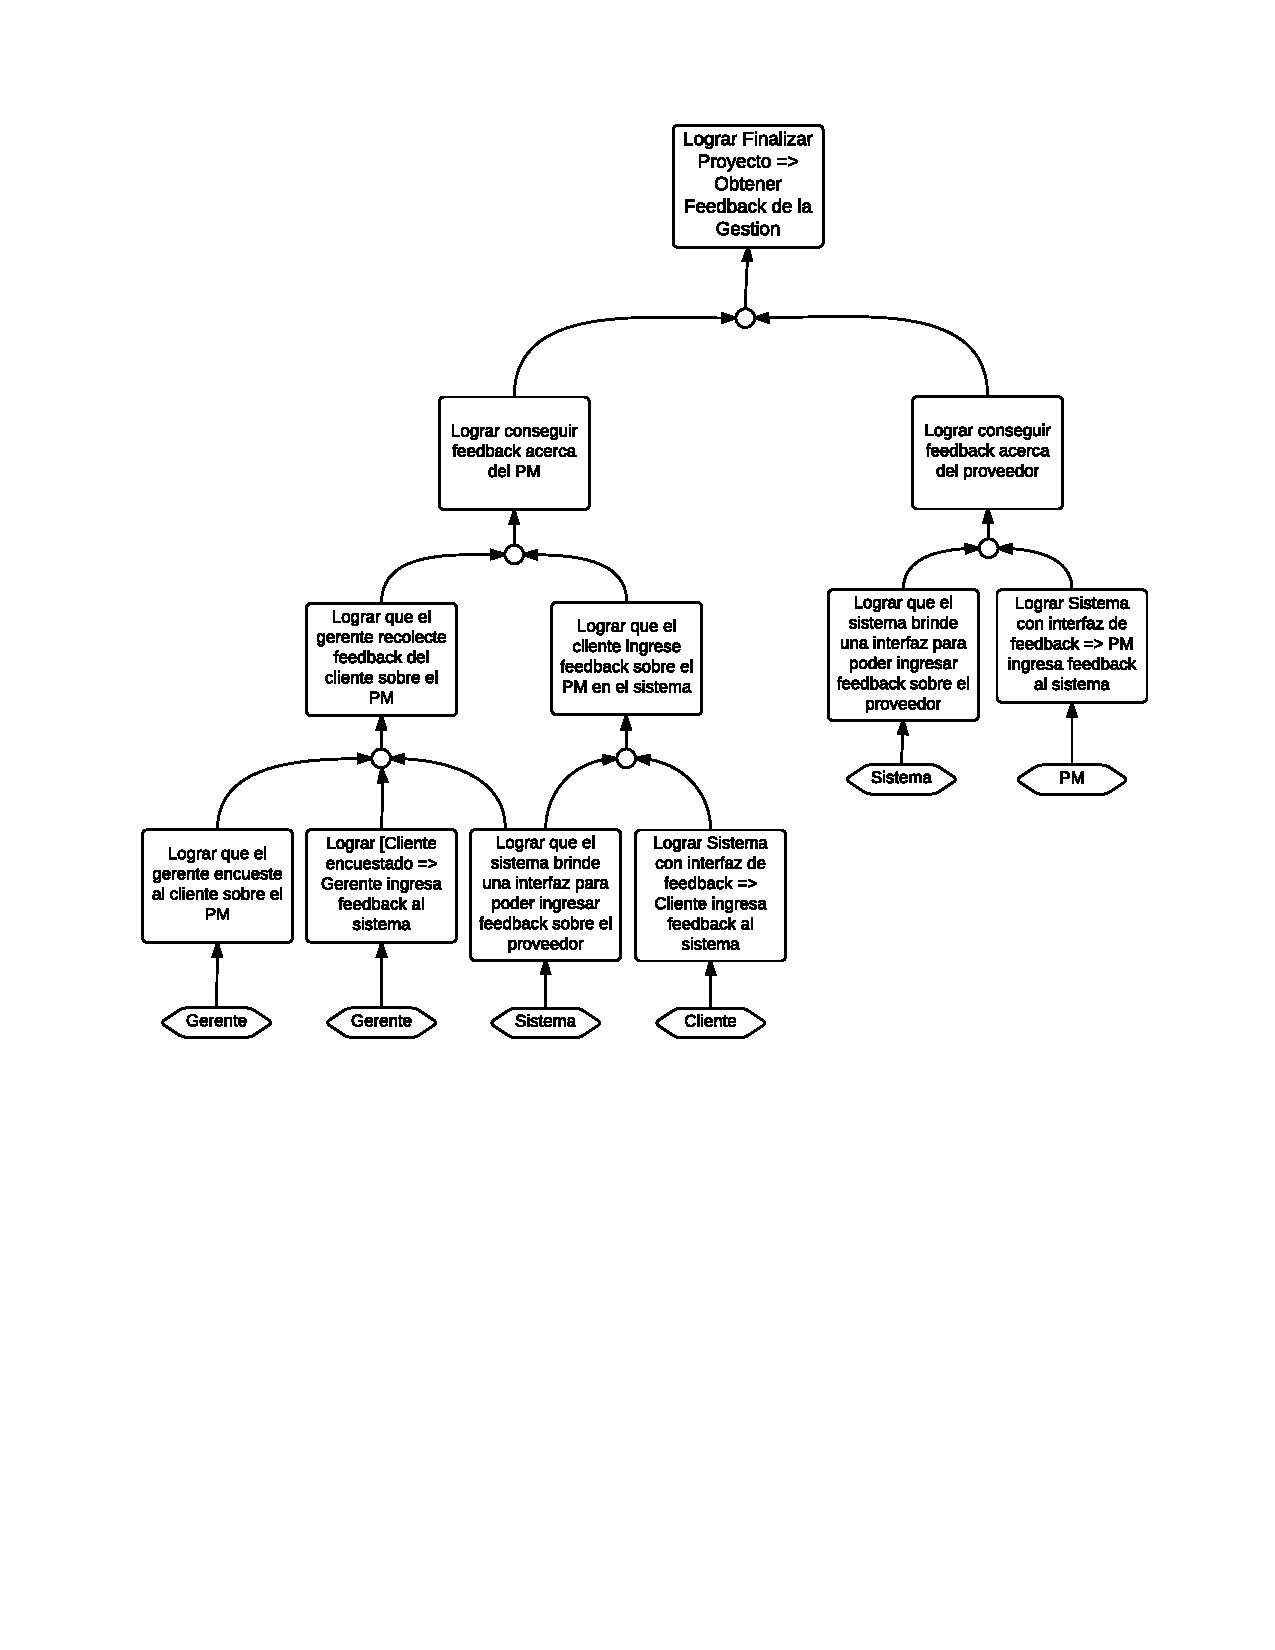
\includegraphics[width=\textwidth, clip=true, trim=15pt 0pt 15pt 0pt]{imagenes/objetivos/objetivos17.pdf}
\end{figure}
